%%% LaTeX Template: Article/Thesis/etc. with colored headings and special fonts
%%%
%%% Source: http://www.howtotex.com/
%%% Feel free to distribute this template, but please keep to referal to http://www.howtotex.com/ here.
%%% February 2011
%%%
%%% Modified January 2016 by CDM

%%%  Preamble
\documentclass[11pt,letterpaper]{article}
\usepackage[margin=1.0in]{geometry}
\usepackage[T1]{fontenc}
\usepackage[bitstream-charter]{mathdesign}
\usepackage[latin1]{inputenc}					
\usepackage{amsmath}						
\usepackage{xcolor}
\usepackage{cite}
\usepackage{hyphenat}
\usepackage{graphicx}
\usepackage{float}
\usepackage{subfigure}
\usepackage{sectsty}
\usepackage[compact]{titlesec} 
\usepackage[tablegrid]{vhistory}
\usepackage{pbox}
\allsectionsfont{\color{accentcolor}\scshape\selectfont}

%%% Definitions
\definecolor{accentcolor}{rgb}{0.0,0.0,0.5} 
\newcommand{\teamname}{Nepster}
\newcommand{\productname}{PocketShelf}
\newcommand{\coursename}{CSE 4317: Senior Design II}
\newcommand{\semester}{Fall 2019}
\newcommand{\docname}{Detailed Design Specification}
\newcommand{\department}{Department of Computer Science \& Engineering}
\newcommand{\university}{The University of Texas at Arlington}
\newcommand{\authors}{Utsab Acharya \\ Sandesh Naga \\ Sudip Kandel \\ Tara Gurung \\ Bhaskar Acharya}

%%% Headers and footers
\usepackage{fancyhdr}
	\pagestyle{fancy}						% Enabling the custom headers/footers
\usepackage{lastpage}	
	% Header (empty)
	\lhead{}
	\chead{}
	\rhead{}
	% Footer
	\lfoot{\footnotesize \teamname \ - \semester}
	\cfoot{}
	\rfoot{\footnotesize page \thepage\ of \pageref{LastPage}}	% "Page 1 of 2"
	\renewcommand{\headrulewidth}{0.0pt}
	\renewcommand{\footrulewidth}{0.4pt}

%%% Change the abstract environment
\usepackage[runin]{abstract}			% runin option for a run-in title
%\setlength\absleftindent{30pt}			% left margin
%\setlength\absrightindent{30pt}		% right margin
\abslabeldelim{\quad}	
\setlength{\abstitleskip}{-10pt}
\renewcommand{\abstractname}{}
\renewcommand{\abstracttextfont}{\color{accentcolor} \small \slshape}	% slanted text

%%% Start of the document
\begin{document}

%%% Cover sheet
{\centering \huge \color{accentcolor} \sc \textbf{\department \\ \university} \par}
\vspace{1 in}
{\centering \huge \color{accentcolor} \sc \textbf{\docname \\ \coursename \\ \semester} \par}
\vspace{0.5 in}
\begin{figure}[h!]
	\centering
   	
\includegraphics[width=0.60\textwidth]{images/Logo.png}
\end{figure}
\vspace{0.5 in}
{\centering \huge \color{accentcolor} \sc \textbf{\teamname \\ \productname} \par}
\vspace{0.5 in}
{\centering \large \sc \textbf{\authors} \par}
\newpage


%\vspace{1 in}
%\centerline{January 13th, 2012}
%\newpage

%%% Revision History
\begin{versionhistory}
  \vhEntry{0.1}{1.01.2016}{SK|UA|SN|BA|TG}{document creation}
  	\vhEntry{0.2}{1.05.2016}{BA|UA|SN|SK|TG}{complete draft}
  	\vhEntry{0.3}{1.12.2016}{SN|UA|BA|SK|TG}{release candidate 1}
  	\vhEntry{1.0}{1.20.2016}{TG|UA|SN|SK|BA}{official release}
  	\vhEntry{1.1}{1.31.2016}{BA|UA|SN|SK|TG}{added design review requests}
\end{versionhistory}
\newpage

%%% Table of contents
\setcounter{tocdepth}{2}
\tableofcontents
\newpage

%%% List of figures and tables (optional)
\listoffigures
\listoftables
\newpage

%%% Document sections
\section{Introduction}
Inventory management is an important part of running business and managing items around us.  Traditional practice of managing items for business cost a lot of time and work force for companies.  Customers become frustrated when the items they're looking for aren't available on the shelf. Bad practice of managing items in our home, school, works etc. cost lots of time because it is hard for us to remember what items are needed and where it is located. Pocket-self is the inventory tracking ISO/Android based mobile application which allow users to keep the items in available space, which is created by the user.We called PocketShelf because the idea behind it, we can carry the inventory application in our pocket and can search items in just a click. The function of the app is user can sign up and login then add items or add shelf or search the items.App can help to find the place where to keep the items in shelf, keeps record of it and help to find the items when customers search for it.  The app can help the customers to find and add the items in the shelf with the help of the items pictures too.  We used Augmented reality as our key feature of the application.  Where user can see the item before they approach to grab it.  Which might be helpful in the sense that it will save the user effort and time spent and they know that they are getting the right thing. Time frame to notify user can be predefined by the user at the time of its entry. Our app use the online database to save every entry by the user and had to be encrypted before it goes to the database,all the data had to flow through the server.  So, user must be online to be able to use the app.  We had PIN protection as an extra feature on the app, where if the user wants not to show the item location to another user using the same app on same device.  Which we found cool feature if the user wants to secure valuable items somewhere in the shelf.The scope of pocketShelf are prioritize inventory, Track all product information, Track sales, sorts in-venture according to manufacture and best by date of the items.  App helps to prioritize inventory on the basic of the customers demand, shape and sizes of items in the shelf.  For example, heavy and big items are preferred in he button of the shelf and small or light items in the top the shelf. App will keep the records of the inventory as well as items in stocks.  Another important feature of the app is track sales.  Update the numbers of the items when add or remove an item from the shelf.  App can sort the inventory according to customer preferences based on attributes of the item.  The app not only keep track of the item but able to sort the items based on the expiration dates and can notify the user if the item is expiring soon.
\section{System Overview}
This is the first sub section that user interacts with. When the user opens the mobile application for the first time details for SignUp is displayed. Then the user enters all the information required for SignUp including all the valid user name and password to create a account. Then an account for the user is created.

\begin{figure}[h!]
	\centering
 	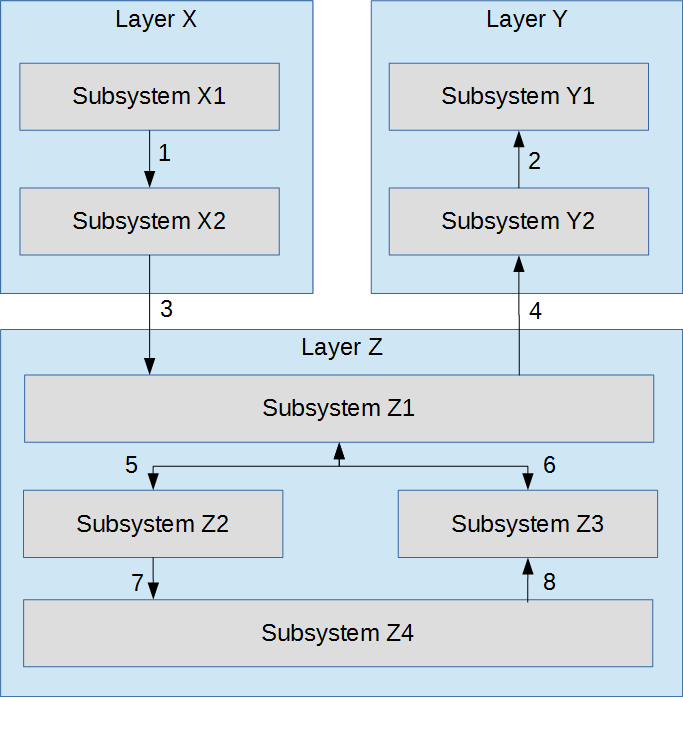
\includegraphics[width=0.90\textwidth]{images/data_flow}
 \caption{System architecture}
\end{figure}

\newpage
%\section{Subsystem Definitions \& Data Flow}
%This section breaks down your layer abstraction to another level of detail. Here you grapically represent the logical subsytems that compose each layer and show the interactions/interfaces between those subsystems. A subsystem can be thought of as a programming unit that implements one of the major functions of the layer. It, therefore, has data elements that serve as source/sinks for other subsystems. The logical data elements that flow between subsystems need to be explicitly defined at this point, beginning with a data flow-like diagram based on the block diagram.

\begin{figure}[h!]
	\centering
 	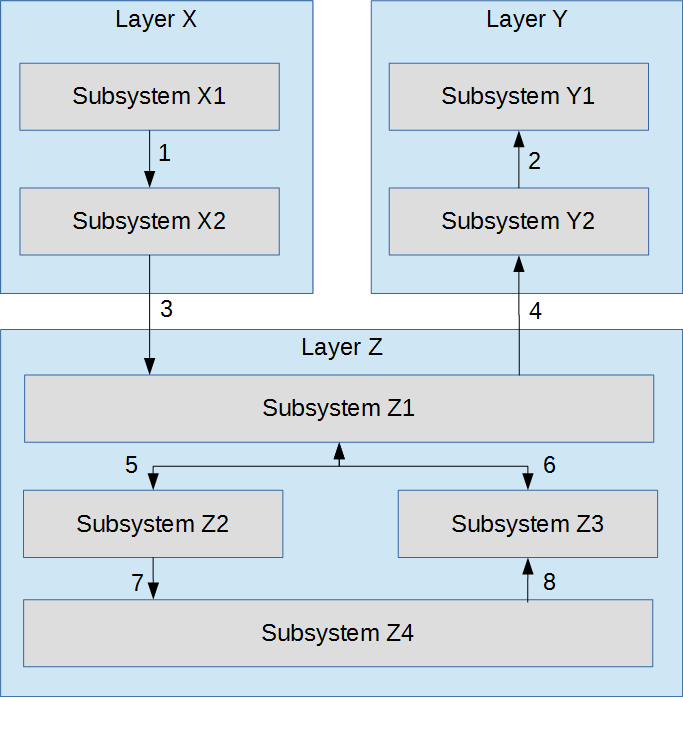
\includegraphics[width=\textwidth]{images/data_flow}
 \caption{A simple data flow diagram}
\end{figure}

\newpage
\section{UI}
UI is the graphic feature of the application mainly responsible for the displaying information and interact with the user. UI consist of login subsystem responsible for taking userid and password from user. Registration subsystem is responsible to take userid, email, password, full name from the user. Add\_Shelf subsystem is responsible for taking the shelf description from the user. Add\_Item is responsible for taking item description from user. Search subsystem is responsible for taking user input via QR code or input text. After any kind input and options chosen by the user UI\_Controller will send all user input and the option chosen by the user to Business\_Controller in Business\_Logic. UI\_Controller also accept the input messages from the Business\_Controller, stating successful completion of the chosen task by the user.

\subsection{Layer Hardware}
Being an android/iOS app, UI will use components underlying hardware for user input and to show output to the user. i.e. user uses phone screen for input and show output in same screen.

\subsection{Layer Operating System}
A description of any operating systems required by the layer.

\subsection{Layer Software Dependencies}
A description of any software dependencies (libraries, frameworks, etc) required by the layer.

\subsection{Subsystem 1}
Descibe at a high level the purpose and basic design of this subsystem. Is it a piece of hardware, a class, a web service, or something else? Note that each of the subsystem items below are meant to be specific to that subystem and not a repeat of anything discussed above for the overall layer.

\begin{figure}[h!]
	\centering
 	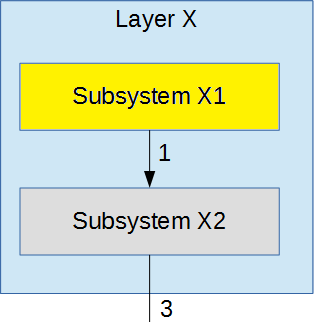
\includegraphics[width=0.60\textwidth]{images/subsystem}
 \caption{Example subsystem description diagram}
\end{figure}

\subsubsection{Subsystem Hardware}
A description of any involved hardware components for the subsystem.

\subsubsection{Subsystem Operating System}
A description of any operating systems required by the subsystem.

\subsubsection{Subsystem Software Dependencies}
A description of any software dependencies (libraries, frameworks, design software for mechanical parts or circuits, etc) required by the subsystem.

\subsubsection{Subsystem Programming Languages}
A description of any programming languages used by the subsystem.

\subsubsection{Subsystem Data Structures}
A description of any classes or other data structures that are worth discussing for the subsystem. For example, data being transmitted from a microcontroller to a PC via USB should be first be assembled into packets. What is the structure of the packets?

\subsubsection{Subsystem Data Processing}
A description of any algorithms or processing strategies that are worth discussing for the subsystem. If you are implementing a well-known algorithm, list it. If it is something unique to this project, discuss it in greater detail.



\newpage
\section{Business Logic}
This is another important layer in our design. This part of the system works as a bridge between the User Interface and the Database of the system. If the data is being received from the UI controller that are coming form different subsections of UI, the Business controller will, depending upon what kind of input it gets, either generate an AR, generate a Qr or does an input validation. The Business Logic will send the data to the data base for more validation and verification or to store the data in database. If Business Logic is getting the instruction to fetch data form Database, then it will contact Database to get particular data, which is then passed on to the UI.

\subsection{Layer Hardware}
A description of any involved hardware components for the layer. For example, if each subsystem is a software process running on an embedded computer, discuss the specifics of that device here. Do not list a hardware component that only exists at the subsystem level (include it in the following sections).

\subsection{Layer Operating System}
iOS/Android

\subsection{Layer Software Dependencies}
This layer is build using ReactNative. Dependencies we needed for this part are
\begin{rand}"dependencies":\\ {
    "expo": "34.0.1",\\
    "expo-barcode-scanner": "6.0.0",\\
    "expo-permissions": "6.0.0",\\
    "firebase": "6.6.0",\\
    "native-base": "2.13.7",\\
    "react": "16.8.3",\\
    "react-dom": "16.8.6",\\
    "react-native": "https://github.com/expo/react-native/archive/sdk-34.0.0.tar.gz",\\
    "react-native-datepicker": "1.7.2",\\
    "react-native-gesture-handler": "1.4.1",\\
    "react-native-search-bar": "3.4.3",\\
    "react-native-simple-radio-button": "2.7.3",\\
    "react-native-vector-icons": "6.6.0",\\
    "react-native-web": "0.11.4",\\
    "react-navigation": "4.0.0",\\
    "react-navigation-stack": "1.5.1",\\
    "reinput": "3.7.1"]\\
\end{rand}
\subsection{Business Controller}
Any kind of data coming and going to Business Logic do so through the Business controller. The data coming to Business Logic will be divided into three different ways, namely AR generation, QR generation or Input Validation related. Depending upon those different input types, Business controller communicates with the Database controller to get particular data or to store that information.

\begin{figure}[h!]
	\centering
 	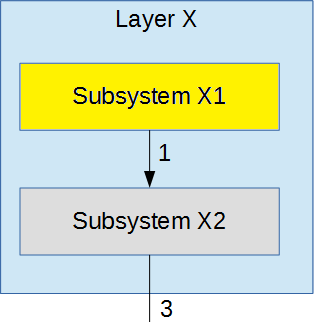
\includegraphics[width=0.60\textwidth]{images/subsystem}
 \caption{Example subsystem description diagram}
\end{figure}

\subsubsection{Subsystem Hardware}
NA

\subsubsection{Subsystem Operating System}
iOS/Andriod

\subsubsection{Subsystem Software Dependencies}
A description of any software dependencies (libraries, frameworks, design software for mechanical parts or circuits, etc) required by the subsystem.

\subsubsection{Subsystem Programming Languages}
JavaScript

\subsubsection{Subsystem Data Structures}
JSON, Array, Union, List.

\subsubsection{Subsystem Data Processing}
Shorting Algorithm was used.

\subsection{AR Generator}
AR generator is the part of Business logic that generates AR when a customer wants to store an item to the shelf. The generated AR is then used when the customer wants to search the item. When the customer wants to search an item, he will scan bar-code or enter manually. Then the program will display the AR right on the bar-code of the item.
\begin{figure}[h!]
	\centering
 	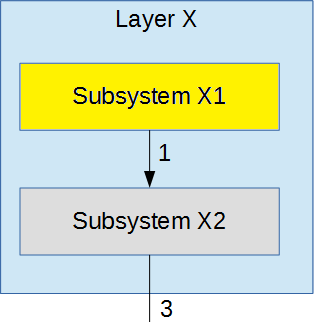
\includegraphics[width=0.60\textwidth]{images/subsystem}
 \caption{Example subsystem description diagram}
\end{figure}

\subsubsection{Subsystem Hardware}
Phone Camera

\subsubsection{Subsystem Operating System}
iOS/Andriod

\subsubsection{Subsystem Software Dependencies}
Phone camera, images available

\subsubsection{Subsystem Programming Languages}
JavaScript

\subsubsection{Subsystem Data Structures}
JSON, Array, Union, List.

\subsubsection{Subsystem Data Processing}
Shorting Algorithm was used.


\subsection{QR Generator}
Based on description of the item customer provides, QR generator generate QR.This QR is then store in the database along with the  description of the item.

\begin{figure}[h!]
	\centering
 	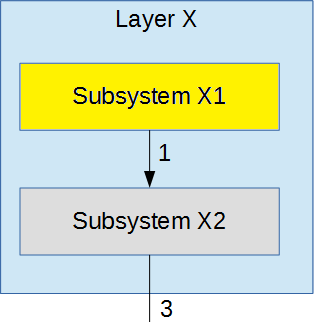
\includegraphics[width=0.60\textwidth]{images/subsystem}
 \caption{Example subsystem description diagram}
\end{figure}

\subsubsection{Subsystem Hardware}
Phone Camera

\subsubsection{Subsystem Operating System}
iOS/Andriod

\subsubsection{Subsystem Software Dependencies}
Phone camera

\subsubsection{Subsystem Programming Languages}
JavaScript

\subsubsection{Subsystem Data Structures}
JSON, Array, Union, List.



\subsection{UI Input Validation}
This section will validate format and types of input from user. It will reject the inputs if user's input is wrong format and suggest the correct format of the input.Provide guidance on how to fix any errors, don't just tell users what they did wrong. It will prevent from unauthorized SQL injection into the data base.

\begin{figure}[h!]
	\centering
 	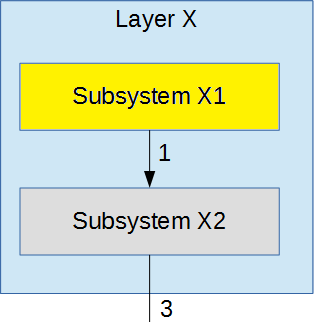
\includegraphics[width=0.60\textwidth]{images/subsystem}
 \caption{Example subsystem description diagram}
\end{figure}

\subsubsection{Subsystem Hardware}
N/A

\subsubsection{Subsystem Operating System}
iOS/Andriod

\subsubsection{Subsystem Software Dependencies}
Phone camera

\subsubsection{Subsystem Programming Languages}
JavaScript

\subsubsection{Subsystem Data Structures}
JSON, Array, Union, List.

\newpage
\section{Database}
This subsection is used when we have to save or retrieve data from the database. When user tries to login, register, add self, add item or search we have to use database. When somebody wants to register for the app, he provides all the information then these information is taken by the DB controller and saved in organized manner. same process occurs for all the other activities like adding self, adding item or login.

\subsection{Layer Hardware}
N/A

\subsection{Layer Operating System}
IOS/Android

\subsection{Layer Software Dependencies}
Firebase, Internal Memory,


\subsection{DB Controller}
This is a type of main controller of the Database system. All the data that needs to be stored in database is first handled by this layer and later stored in the database. When any of the other layer send data to the database layer, first database layer takes the information and figures out what type of data is provided and what to do with the given data.

\begin{figure}[h!]
	\centering
 	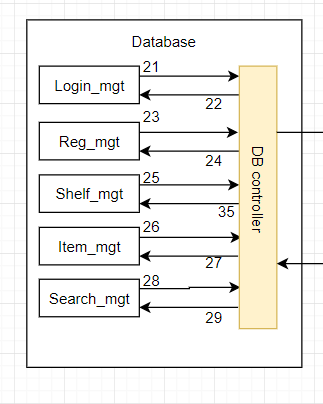
\includegraphics[width=0.60\textwidth]{images/dbcontroller}
 \caption{DB Controller description diagram}
\end{figure}

\subsubsection{DB Controller Hardware}
Internal Memory

\subsubsection{DB Controller Operating System}
iOS/Android

\subsubsection{DB Controller Software Dependencies}
\begin{rand}"dependencies":\\ {
    "expo": "34.0.1",\\    \
    "expo-permissions": "6.0.0",\\
    "firebase": "6.6.0",\\
    "react": "16.8.3",\\
    "react-native": "https://github.com/expo/react-native/archive/sdk-34.0.0.tar.gz",\\
    "react-navigation-stack": "1.5.1",\\
\end{rand}

\subsubsection{DB Controller Programming Languages}
JavaScript

\subsubsection{DB Controller Data Structures}
JSON, Array, Objects

\subsubsection{DB Controller Data Processing}
Depending upon the data provided by the user, data will be sent to the subsystems of database ie. login\_mgt, Reg\_mgt, Shelf\_mgt, Item\_mgt, Search\_mgt.
According to the query of the user database willthe subsystems ie. login\_mgt, Reg\_mgt, Shelf\_mgt, Item\_mgt, Search\_mgt and help user in validation of user and fetching of data.


\subsection{Login Mgt}
This subsection of database just deals with the login information. User first registers for the account in the mobile application. Then when he wants to use the app he will provide the user name and password for the app. Then the login management layer handles all the data. It checks if the user name and password provided by the user exists in database or not. It should allow user to login if the combination of user name and password exists else it should deny user from using the application itself.

\begin{figure}[h!]
	\centering
 	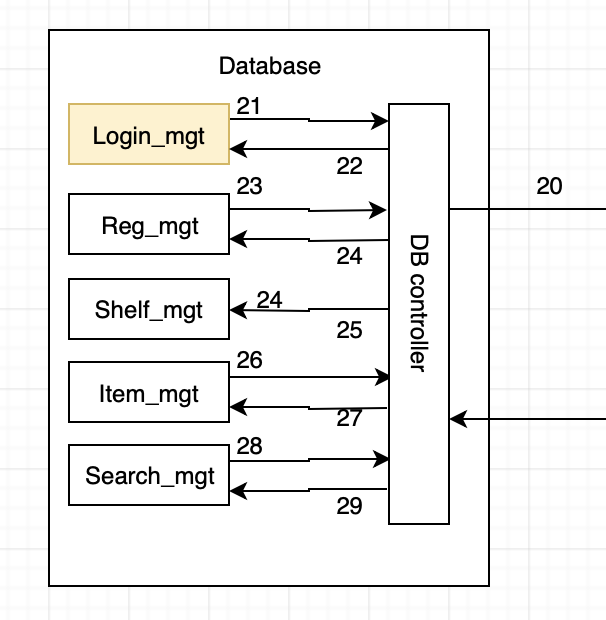
\includegraphics[width=0.60\textwidth]{images/loginmgt}
 \caption{Login mgt description diagram}
\end{figure}

\subsubsection{Login Mgt Hardware}
Internal Memory

\subsubsection{Login Mgt Operating System}
iOS/Android

\subsubsection{Login Mgt Software Dependencies}
\begin{rand}"dependencies":\\ {
    "expo": "34.0.1",\\
    "expo-permissions": "6.0.0",\\
    "firebase": "6.6.0",\\
    "react": "16.8.3",\\ "react-native-gesture-handler": "1.4.1",\\
    "react-navigation-stack": "1.5.1",\\
    "reinput": "3.7.1"]\\
\end{rand}

\subsubsection{Login Mgt Programming Languages}
JavaScript

\subsubsection{Login Mgt Data Structures}
JSON, Array, Objects

\subsubsection{Login Mgt Data Processing}
Depending upon the data provided by the user, data will be sent to the subsystem ie. login\_mgt. Login\_mgt will then validate the user if the username and password is correct. 
This will return a boolean result if the user is authorized or not.



\subsection{Register Mgt}
This subsection of the database deals with registration data like first name, last name, DOB,etc. When user provides the information it is validated for SQL injection and passed into the register management. Then the data is stored in database in organized manner by the register management subsystem.

\begin{figure}[h!]
	\centering
 	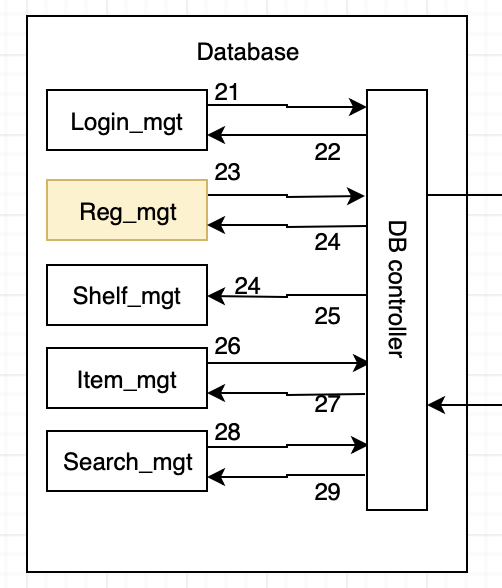
\includegraphics[width=0.60\textwidth]{images/regmgt}
 \caption{Register mgt description diagram}
\end{figure}


\subsubsection{Register Mgt Hardware}
Internal Memory

\subsubsection{Register Mgt Operating System}
iOS/Android

\subsubsection{Register Mgt Software Dependencies}
\begin{rand}"dependencies":\\ {
    "expo": "34.0.1",\\
    "expo-permissions": "6.0.0",\\
    "firebase": "6.6.0",\\
    "react": "16.8.3",\\ "react-native-gesture-handler": "1.4.1",\\
    "react-navigation-stack": "1.5.1",\\
    "reinput": "3.7.1"]\\
\end{rand}

\subsubsection{Register Mgt Programming Languages}
JavaScript

\subsubsection{Register Mgt Data Structures}
JSON, Array, Objects

\subsubsection{Register Mgt Data Processing}
Depending upon the data provided by the user, data will be sent to the subsystem ie. Register\_mgt. Register\_mgt will then validate the user if the username and password is correct. 
This will return a boolean result if the user is authorized or not.

\subsection{Item mgt}
This subsystem of the database is used whenever user wants to add or remove item from the database. When user provides the data for adding or removing the item, then the DB controller takes the input at first and then passes it to the item Mgmt. Then the layer takes the input value and make necessary change ie. add or remove the item accordingly.

\begin{figure}[h!]
	\centering
 	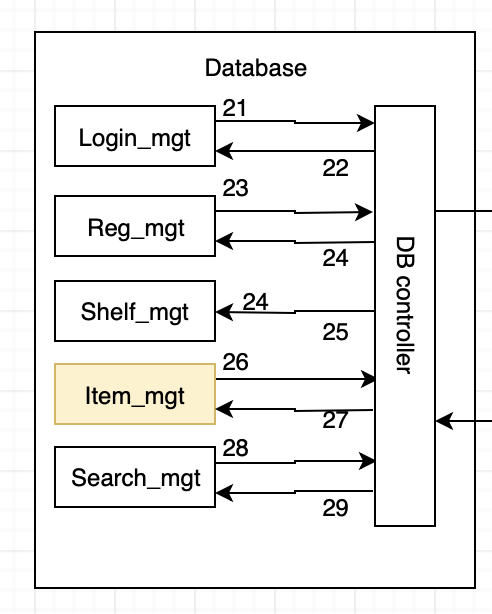
\includegraphics[width=0.60\textwidth]{images/itemmgt}
 \caption{Item mgt description diagram}
\end{figure}

\subsubsection{Item Mgt Hardware}
Internal Memory

\subsubsection{Item Mgt Operating System}
IOS/Android


























































\subsubsection{Item Mgt Software Dependencies}
\begin{rand}"dependencies":\\ {
    "expo": "34.0.1",\\
    "expo-permissions": "6.0.0",\\
    "firebase": "6.6.0",\\
    "react": "16.8.3",\\ "react-native-gesture-handler": "1.4.1",\\
    "react-navigation-stack": "1.5.1",\\
    "reinput": "3.7.1"]\\
\end{rand}

\subsubsection{Item Mgt Programming Languages}
JavaScript

\subsubsection{Item Mgt Data Structures}
JSON, Array, Objects

\subsubsection{Item Mgt Data Processing}
Depending upon the data provided by the user, data will stored in the logged in user's database.

\subsection{Search mgt}
This Sub System deals with taking the item description from user and it searches for the item. Variety of options are provided for searching the item. User can use the camera in the cellphone to scan the QR generated for the specific item or users will also be able to search the item by their names.

\begin{figure}[h!]
	\centering
 	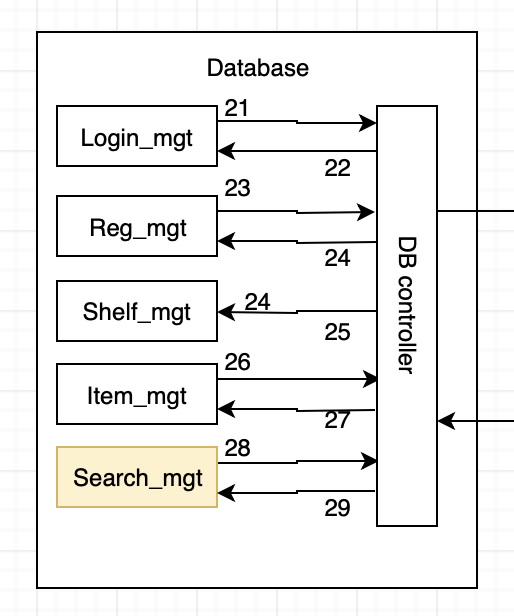
\includegraphics[width=0.60\textwidth]{images/searchmgt}
 \caption{Search mgt description diagram}
\end{figure}

\subsubsection{Search Mgt Hardware}
Phone display

\subsubsection{Search Mgt Operating System}
IOS/Android

\subsubsection{Search Mgt Software Dependencies}
\begin{rand}"dependencies":\\ {
    "expo": "34.0.1",\\
    "expo-permissions": "6.0.0",\\
    "firebase": "6.6.0",\\
    "react": "16.8.3",\\ "react-native-gesture-handler": "1.4.1",\\
    "react-navigation-stack": "1.5.1",\\
    "reinput": "3.7.1"]\\
\end{rand}

\subsubsection{Search Mgt Programming Languages}
JavaScript

\subsubsection{Search Mgt Data Structures}
 Array, Objects, Union

\subsubsection{Search Mgt Data Processing}
Depending upon the data provided by the user, data will be retrieved from logged in user's database.


\newpage
\section{Appendix A}
Include any additional documents (CAD design, circuit schematics, etc) as an appendix as necessary.
\newpage

%%% References
\bibliographystyle{plain}
\bibliographystyle{reference/IEEEtran_custom}
\bibliography{reference/refs}{}

\end{document}